%
\documentclass[journal,12pt,twocolumn]{IEEEtran}
%
\usepackage{setspace}
\usepackage{gensymb}
\usepackage{bm}
\usepackage{xcolor}
\usepackage{caption}
%\usepackage{subcaption}
%\doublespacing
\singlespacing
\usepackage{enumitem}
%\usepackage{multicol}
%\usepackage{graphicx}
%\usepackage{amssymb}
%\usepackage{relsize}
\usepackage[cmex10]{amsmath}
\usepackage{mathtools}
%\usepackage{amsthm}
%\interdisplaylinepenalty=2500
%\savesymbol{iint}
%\usepackage{txfonts}
%\restoresymbol{TXF}{iint}
%\usepackage{wasysym}
\usepackage{amsthm}
\usepackage{mathrsfs}
\usepackage{txfonts}
\usepackage{stfloats}
\usepackage{cite}
\usepackage{cases}
\usepackage{subfig}
%\usepackage{xtab}
\usepackage{longtable}
\usepackage{multirow}
%\usepackage{algorithm}
%\usepackage{algpseudocode}
\usepackage{enumitem}
\usepackage{mathtools}
\usepackage{iithtlc}
%\usepackage[framemethod=tikz]{mdframed}
\usepackage{listings}
    \usepackage[latin1]{inputenc}                                 %%
    \usepackage{color}                                            %%
    \usepackage{array}                                            %%
    \usepackage{longtable}                                        %%
    \usepackage{calc}                                             %%
    \usepackage{multirow}                                         %%
    \usepackage{hhline}                                           %%
    \usepackage{ifthen}                                           %%
  %optionally (for landscape tables embedded in another document): %%
    \usepackage{lscape}     

%\usepackage{stmaryrd}


%\usepackage{wasysym}
%\newcounter{MYtempeqncnt}
\DeclareMathOperator*{\Res}{Res}
%\renewcommand{\baselinestretch}{2}
\renewcommand\thesection{\arabic{section}}
\renewcommand\thesubsection{\thesection.\arabic{subsection}}
\renewcommand\thesubsubsection{\thesubsection.\arabic{subsubsection}}

\renewcommand\thesectiondis{\arabic{section}}
\renewcommand\thesubsectiondis{\thesectiondis.\arabic{subsection}}
\renewcommand\thesubsubsectiondis{\thesubsectiondis.\arabic{subsubsection}}

% correct bad hyphenation here
\hyphenation{op-tical net-works semi-conduc-tor}

\def\inputGnumericTable{}  

\lstset{
%language=python,
frame=single, 
breaklines=true,
columns=fullflexible
}
\newcommand\bigzero{\makebox(0,0){\text{\huge0}}}
%\lstset{
	%%basicstyle=\small\ttfamily\bfseries,
	%%numberstyle=\small\ttfamily,
	%language=Octave,
	%backgroundcolor=\color{white},
	%%frame=single,
	%%keywordstyle=\bfseries,
	%%breaklines=true,
	%%showstringspaces=false,
	%%xleftmargin=-10mm,
	%%aboveskip=-1mm,
	%%belowskip=0mm
%}

%\surroundwithmdframed[width=\columnwidth]{lstlisting}


\begin{document}
%

\theoremstyle{definition}
\newtheorem{theorem}{Theorem}[section]
\newtheorem{problem}{Problem}
\newtheorem{proposition}{Proposition}[section]
\newtheorem{lemma}{Lemma}[section]
\newtheorem{corollary}[theorem]{Corollary}
\newtheorem{example}{Example}[section]
\newtheorem{definition}{Definition}[section]
%\newtheorem{algorithm}{Algorithm}[section]
%\newtheorem{cor}{Corollary}
\newcommand{\BEQA}{\begin{eqnarray}}
\newcommand{\EEQA}{\end{eqnarray}}
\newcommand{\define}{\stackrel{\triangle}{=}}

\bibliographystyle{IEEEtran}
%\bibliographystyle{ieeetr}

\providecommand{\nCr}[2]{\,^{#1}C_{#2}} % nCr
\providecommand{\nPr}[2]{\,^{#1}P_{#2}} % nPr
\providecommand{\mbf}{\mathbf}
\providecommand{\pr}[1]{\ensuremath{\Pr\left(#1\right)}}
\providecommand{\qfunc}[1]{\ensuremath{Q\left(#1\right)}}
\providecommand{\sbrak}[1]{\ensuremath{{}\left[#1\right]}}
\providecommand{\lsbrak}[1]{\ensuremath{{}\left[#1\right.}}
\providecommand{\rsbrak}[1]{\ensuremath{{}\left.#1\right]}}
\providecommand{\brak}[1]{\ensuremath{\left(#1\right)}}
\providecommand{\lbrak}[1]{\ensuremath{\left(#1\right.}}
\providecommand{\rbrak}[1]{\ensuremath{\left.#1\right)}}
\providecommand{\cbrak}[1]{\ensuremath{\left\{#1\right\}}}
\providecommand{\lcbrak}[1]{\ensuremath{\left\{#1\right.}}
\providecommand{\rcbrak}[1]{\ensuremath{\left.#1\right\}}}
\theoremstyle{remark}
\newtheorem{rem}{Remark}
\newcommand{\sgn}{\mathop{\mathrm{sgn}}}
\providecommand{\abs}[1]{\left\vert#1\right\vert}
\providecommand{\res}[1]{\Res\displaylimits_{#1}} 
\providecommand{\norm}[1]{\left\Vert#1\right\Vert}
\providecommand{\mtx}[1]{\mathbf{#1}}
\providecommand{\mean}[1]{E\left[ #1 \right]}
\providecommand{\fourier}{\overset{\mathcal{F}}{ \rightleftharpoons}}
%\providecommand{\hilbert}{\overset{\mathcal{H}}{ \rightleftharpoons}}
\providecommand{\system}{\overset{\mathcal{H}}{ \longleftrightarrow}}
	%\newcommand{\solution}[2]{\textbf{Solution:}{#1}}
\newcommand{\solution}{\noindent \textbf{Solution: }}
\newcommand{\myvec}[1]{\ensuremath{\begin{pmatrix}#1\end{pmatrix}}}
\providecommand{\dec}[2]{\ensuremath{\overset{#1}{\underset{#2}{\gtrless}}}}
\providecommand{\gauss}[2]{\mathcal{N}\ensuremath{\left(#1,#2\right)}}

%\numberwithin{equation}{subsection}
\numberwithin{equation}{section}
%\numberwithin{equation}{problem}
%\numberwithin{problem}{subsection}
\numberwithin{problem}{section}
%\numberwithin{definition}{subsection}
\makeatletter
\@addtoreset{figure}{problem}
\makeatother
\makeatletter
\@addtoreset{table}{problem}
\makeatother

\let\StandardTheFigure\thefigure
\let\StandardTheTable\thetable
\let\vec\mathbf

%\renewcommand{\thefigure}{\theproblem.\arabic{figure}}
\renewcommand{\thefigure}{\theproblem}
\renewcommand{\thetable}{\theproblem}
%\numberwithin{figure}{section}

%\numberwithin{figure}{subsection}

\def\putbox#1#2#3{\makebox[0in][l]{\makebox[#1][l]{}\raisebox{\baselineskip}[0in][0in]{\raisebox{#2}[0in][0in]{#3}}}}
     \def\rightbox#1{\makebox[0in][r]{#1}}
     \def\centbox#1{\makebox[0in]{#1}}
     \def\topbox#1{\raisebox{-\baselineskip}[0in][0in]{#1}}
     \def\midbox#1{\raisebox{-0.5\baselineskip}[0in][0in]{#1}}

\vspace{3cm}


\title{%Convex Optimization in Python
	\logo{
	Support Vector Machines
	}
}
%\title{
%	\logo{Matrix Analysis through Octave}{\begin{center}\includegraphics[scale=.24]{tlc}\end{center}}{}{HAMDSP}
%}


% paper title
% can use linebreaks \\ within to get better formatting as desired
%\title{Matrix Analysis through Octave}
%
%
% author names and IEEE memberships
% note positions of commas and nonbreaking spaces ( ~ ) LaTeX will not break
% a structure at a ~ so this keeps an author's name from being broken across
% two lines.
% use \thanks{} to gain access to the first footnote area
% a separate \thanks must be used for each paragraph as LaTeX2e's \thanks
% was not built to handle multiple paragraphs
%

\author{G V V Sharma$^{*}$% <-this % stops a space
\thanks{* The authors are with the Department
of Electrical Engineering, Indian Institute of Technology, Hyderabad
502285 India e-mail:  gadepall@iith.ac.in.}% <-this % stops a space
%\thanks{J. Doe and J. Doe are with Anonymous University.}% <-this % stops a space
%\thanks{Manuscript received April 19, 2005; revised January 11, 2007.}}
}
% note the % following the last \IEEEmembership and also \thanks - 
% these prevent an unwanted space from occurring between the last author name
% and the end of the author line. i.e., if you had this:
% 
% \author{....lastname \thanks{...} \thanks{...} }
%                     ^------------^------------^----Do not want these spaces!
%
% a space would be appended to the last name and could cause every name on that
% line to be shifted left slightly. This is one of those "LaTeX things". For
% instance, "\textbf{A} \textbf{B}" will typeset as "A B" not "AB". To get
% "AB" then you have to do: "\textbf{A}\textbf{B}"
% \thanks is no different in this regard, so shield the last } of each \thanks
% that ends a line with a % and do not let a space in before the next \thanks.
% Spaces after \IEEEmembership other than the last one are OK (and needed) as
% you are supposed to have spaces between the names. For what it is worth,
% this is a minor point as most people would not even notice if the said evil
% space somehow managed to creep in.



% The paper headers
%\markboth{Journal of \LaTeX\ Class Files,~Vol.~6, No.~1, January~2007}%
%{Shell \MakeLowercase{\textit{et al.}}: Bare Demo of IEEEtran.cls for Journals}
% The only time the second header will appear is for the odd numbered pages
% after the title page when using the twoside option.
% 
% *** Note that you probably will NOT want to include the author's ***
% *** name in the headers of peer review papers.                   ***
% You can use \ifCLASSOPTIONpeerreview for conditional compilation here if
% you desire.




% If you want to put a publisher's ID mark on the page you can do it like
% this:
%\IEEEpubid{0000--0000/00\$00.00~\copyright~2007 IEEE}
% Remember, if you use this you must call \IEEEpubidadjcol in the second
% column for its text to clear the IEEEpubid mark.



% make the title area
\maketitle

\tableofcontents

\renewcommand{\thefigure}{\theenumi}
\renewcommand{\thetable}{\theenumi}

\begin{abstract}
This manual provides an introduction to SVM.
\end{abstract}

\section{Reflection}
\begin{enumerate}[label=\thesection.\arabic*,ref=\thesection.\theenumi]

\item Find the distance of $\vec{x}_1 = \myvec{2 \\ 1}$ from the line
\begin{align}
\myvec{3 & 4}\vec{x} + 5 = 0
\end{align}

\item Show that the distance of the point  $\vec{x}_1$ from the line 
\begin{align}
\vec{n}^T\vec{x} +c = 0, \quad \norm{\vec{n}} = 1
\end{align}
is
\begin{align}
M = \abs{\vec{n}^T\vec{x}_1 +c}
%P = \cbrak{\vec{x}:f\brak{\vec{x}}=\vec{n}^T\vec{x} +c = 0}, \quad \norm{\vec{n}} = 1
\end{align}

\item Find the reflection $\vec{x_2}$ of $\vec{x_1}$.
\item Define
\begin{align}
f\brak{\vec{x}}=\vec{n}^T\vec{x} +c
%P = \cbrak{\vec{x}:f\brak{\vec{x}}=\vec{n}^T\vec{x} +c = 0}, \quad \norm{\vec{n}} = 1
\end{align}
\item Compute $f\brak{\vec{x_1}}$ and $f\brak{\vec{x_2}}$.  Comment.

\end{enumerate}

\section{Optimization Problem}
\begin{enumerate}[label=\thesection.\arabic*,ref=\thesection.\theenumi]

\item Suppose $\brak{\vec{x_1},y_1}$ and $\brak{\vec{x_2},y_2}$  are i/o data for a system where $y_1, y_2 \in 
\cbrak{1,-1}$. If you want 
to find $\vec{n},c$ from the given dataset, how will formulate the equivalent 
optimization 
problem?
\\
\solution
 Consider the optimization problem
\begin{align}
\label{eq:m_opt}
\max_{\vec{n},c}M
\\
\label{eq:m_opt_const1}
\text{s.t} \quad y_1\brak{\vec{x}_1^T\vec{n}+c} &\ge M
\\
\label{eq:m_opt_const2}
y_2\brak{\vec{x}_2^T\vec{n}+c} &\ge M
\\
\norm{\vec{n}} &= 1
\label{eq:m_opt_end}
\end{align}
\item The {\em signum} function is defined as
\begin{align}
\sgn(z) = 
\begin{cases}
1  & z > 0
\\
0  & z = 0
\\
-1  & z < 0
\end{cases}
\end{align}
Show that
%
\begin{align}
\sgn(\vec{x}^T\vec{n}+c) = \sgn(\vec{x}^T\vec{w}+d)
\end{align}
%
where
\begin{align}
\begin{split}
\vec{w} = \frac{\vec{n}}{M}, 
d = \frac{c}{M}, M >0
\end{split}
\label{eq:opt_ntow}
\end{align}

\item Show that \eqref{eq:m_opt}-\eqref{eq:m_opt_end} can be reformulated as
%
\begin{align}
\label{eq:opt_w}
\min_{\vec{w},d}\frac{1}{2}\norm{\vec{w}}^2
\\
\text{s.t} \quad  y_i\brak{\vec{x}_i^T\vec{w}+d} \ge&1
\end{align}
\solution From \eqref{eq:opt_ntow},
\begin{align}
\vec{w} &= \frac{\vec{n}}{M} \implies 
 \norm{\vec{w}} = \frac{\norm{\vec{n}}}{M} 
\\
\implies M &= \frac{1}{\norm{\vec{w}}} \because \norm{n} = 1
\end{align}
Thus, 
\begin{align}
\max_{\vec{n},c}M = \max_{\vec{w},d}\frac{1}{\norm{\vec{w}}}=\min_{\vec{w},d}\norm{\vec{w}}.
\end{align}
Also, \eqref{eq:m_opt_const1}-\eqref{eq:m_opt_const2} become
\begin{align}
y_i\brak{\vec{x}_i^T\vec{w}+d} \ge&1
\end{align}
%
\end{enumerate}
\section{Solver}
\begin{enumerate}[label=\thesection.\arabic*,ref=\thesection.\theenumi]

\item Solve \eqref{eq:opt_w} using {\em cvxpy/cvxopt} for $\vec{x}_1=\myvec{2 \\ 1},y_1=1$ and 
$\vec{x}_2=\myvec{0.8 \\ -0.6},y_2=-1$.
\\
\solution  From the given information, the constraints in \eqref{eq:opt_w} become
\begin{align}
\label{eq:data_constraints1}
\myvec{2 & 1}\vec{w}+d \ge&1
\\
\myvec{0.8 & -0.6}\vec{w}+d \le&-1
\label{eq:data_constraints2}
\end{align}
%
The following code results in 
\begin{align}
\vec{w}_{opt} = \myvec{0.6 & 0.8}, d_{opt} = 1, 
\norm{\vec{w}_{opt}}^2 = 1
\end{align}
\lstinputlisting{./codes/svm_cvx.py}
\item Provide a graphical representation for  \eqref{eq:opt_w} 
\\
\solution The following code plots Fig. \ref{fig:svm_graph}.  The 
constraint lines in \eqref{eq:data_constraints1}-\eqref{eq:data_constraints2} are plotted for $d = 0, 
0.5$ 
and 1.  The circles $\norm{\vec{w}}^2 = r^2$ are plotted for $r = 1,2$ and 
3. The smalles circle that satisfies the constraints is obtained when $d = 
1$
\begin{lstlisting}
wget https://raw.githubusercontent.com/gadepall/EE1390/master/manuals/svm/codes/svm_graph.py
\end{lstlisting}
%
\begin{figure}[!ht]
\centering
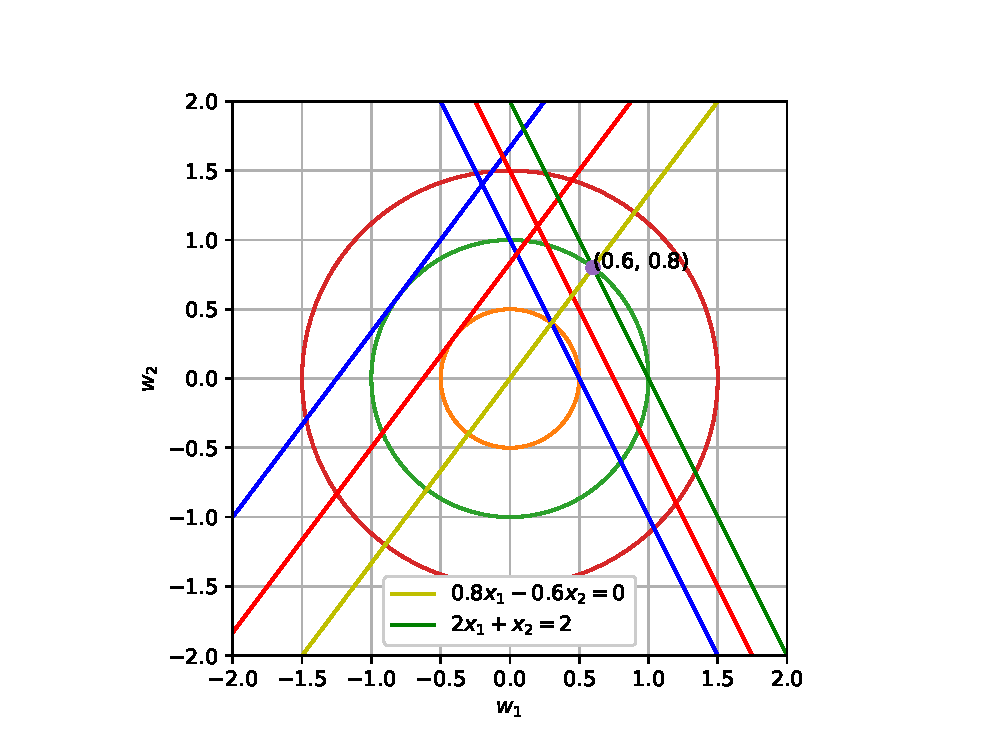
\includegraphics[width=\columnwidth]{./figs/svm_graph.eps}
\caption{}
\label{fig:svm_graph}
\end{figure}
%$\brak{\vec{x}_1,y_1}=\sbrak{\myvec{2 \\ 1},1}$ and 
%$\brak{\vec{x}_2,y_2}=\sbrak{\myvec{0.8 \\ -0.6},-1}$ graphically.
\end{enumerate}
\section{KKT Solution}
\begin{enumerate}[label=\thesection.\arabic*,ref=\thesection.\theenumi]

\item Show that the Lagrangian for \eqref{eq:opt_w}  can be expressed as
\begin{multline}
\label{eq:opt_lagrange}
L_p\brak{\vec{w},\bm{\alpha},d}
= \frac{1}{2}\norm{\vec{w}}^2 
\\
-
\bm{\alpha}^T 
\brak{\myvec{y_1\vec{x}_1& y_2\vec{x}_2}^T\vec{w}+d\myvec{y_1 \\ y_2}-\myvec{1\\1} }
\end{multline}
where
\begin{align}
\bm{\alpha} = \myvec{\alpha_1 \\ \alpha_2}
\end{align}
are the Lagrange multipliers.
\\
\solution
The Lagrangian is given by, 
\begin{multline}
L_p\brak{\vec{w},\bm{\alpha},d}= \frac{1}{2}\norm{\vec{w}}^2 
\\
- 
\sum_{i=1}^{2}\alpha_i\cbrak{y_i\brak{\vec{x}_i^T\vec{w}+d} -1}
%\\
%= \frac{1}{2}\norm{\vec{w}}^2 
%\\
%-
%\bm{\alpha}^T 
%\brak{\myvec{y_1\vec{x}_1& y_2\vec{x}_2}^T\vec{w}+\brak{d-1}\myvec{y_1 \\ y_2} }
\end{multline}
which can be simplified to obtain \eqref{eq:opt_lagrange}
%
\item Show that the stationarity condtion  with respect to $\vec{w}$ yields
\begin{align}
 \myvec{\vec{I} & -\myvec{y_1\vec{x}_1 & y_2\vec{x}_2} & \vec{0}}\myvec{\vec{w} 
\\\bm{\alpha} \\ d} &= 0
\label{eq:opt_stationw}
\end{align}
%
\solution From the stationarity condition
\begin{align}
\nabla_{\vec{w}} L_p\brak{\vec{w},\bm{\alpha},d} &= 0 
\\
%\implies  \vec{w}
%-
%\myvec{\myvec{y_1\vec{x}_1& y_2\vec{x}_2} \bm{\alpha}
% &= 0
%\\
\text{or,}\quad \vec{w}- 
\myvec{y_1\vec{x}_1 & y_2\vec{x}_2}\bm{\alpha} &= 0
\end{align}
resulting in \eqref{eq:opt_stationw}.
\item Show that the stationarity condition with respect to $\bm{\alpha}$ yields
\begin{align}
%%\label{eq:opt_station}
%\nabla_{\bm{\alpha}} L_{p}\brak{\vec{w},\bm{\alpha},d} &= 0 
%\\
%\implies  
%\myvec{y_1\vec{x}_1& y_2\vec{x}_2}^T\vec{w}+\brak{d-1}\myvec{y_1 \\ y_2}  &= 0
%%\vec{x}_i^T\vec{w}+d -1&= 0 
%\\
%\text{or,}\quad 
\myvec{\myvec{y_1\vec{x}_1&y_2\vec{x}_2}^T & \vec{0} & \myvec{y_1 \\ y_2}}\myvec{\vec{w}\\\bm{\alpha} \\ d} 
&= 
\myvec{1\\1} 
\label{eq:opt_station_alpha}
\end{align}
\solution 
\begin{align}
%\label{eq:opt_station}
\nabla_{\bm{\alpha}} L_{p}\brak{\vec{w},\bm{\alpha},d} &= 0 
\\
\implies  
\myvec{y_1\vec{x}_1& y_2\vec{x}_2}^T\vec{w}+d\myvec{y_1 \\ y_2}-\myvec{1\\1}  &= 0
%\vec{x}_i^T\vec{w}+d -1&= 0 
%\\
%\text{or,}\quad 
%\myvec{\myvec{\vec{x}_1&\vec{x}_2}^T & \vec{0} & \myvec{1 \\ 1}}\myvec{\vec{w}\\\bm{\alpha} \\ d} 
%&= 
%\myvec{1\\1} 
\end{align}
after simplification resulting in \eqref{eq:opt_station_alpha}
%
\item Find the stationarity condition with respect to $d$.
\\
\solution
\begin{align}
%\label{eq:opt_station}
\nabla_{d} L_{p}\brak{\vec{w},\bm{\alpha},d} &= 0 
\\
\implies  
\myvec{y_1&y_2} \bm{\alpha}&=0
\\
\text{or,}\quad \myvec{\vec{0}& \myvec{y_1&y_2} & 0} \myvec{\vec{w} 
\\\bm{\alpha} \\ d}&=0
\label{eq:opt_stationd}
\end{align}
%
\item Obtain a matrix equation  for $\vec{w}$ and $d$.
\\
\solution 
\eqref{eq:opt_stationw}
\eqref{eq:opt_station_alpha} and 
\eqref{eq:opt_stationd} can be stacked into a single matrix equation as
{\small
\begin{align}
\label{eq:svm_matrix}
\myvec{\vec{I} & -\myvec{y_1\vec{x}_1 & y_2\vec{x}_2} & \vec{0}
\\
\myvec{y_1\vec{x}_1&y_2\vec{x}_2}^T & \vec{0} & \myvec{y_1 \\ y_2}
\\
\vec{0}& \myvec{y_1&y_2} & 0} 
\myvec{\vec{w} 
\\\bm{\alpha} \\ d}=\myvec{0 \\ 0 \\1\\1\\0} 
\end{align}
}
\item Find the optimal values of $\vec{w}$ and $d$ by solving \eqref{eq:svm_matrix} using python.
\\
\solution
\begin{lstlisting}
wget https://github.com/gadepall/EE1390/raw/master/manuals/svm/codes/svm_matrix.py
\end{lstlisting}

\end{enumerate}
\section{Duality}
\begin{enumerate}[label=\thesection.\arabic*,ref=\thesection.\theenumi]

\item Substitute \eqref{eq:opt_stationw}
%\eqref{eq:opt_station_alpha} and 
and \eqref{eq:opt_stationd}
in the primal function to obtain the Lagrangian 
(Wolfe) dual objective function $L_D$.  
\\
\solution From \eqref{eq:opt_stationw}
\begin{align}
\vec{w} &= \myvec{y_1\vec{x}_1 & y_2\vec{x}_2}\bm{\alpha} 
\\
\implies \vec{w}^T\vec{w} &= \bm{\alpha}^T \myvec{y_1\vec{x}_1^T \\ y_2\vec{x}_2^T}\myvec{y_1\vec{x}_1 & 
y_2\vec{x}_2}\bm{\alpha} 
\\
\text{and } \bm{\alpha}^T &
\myvec{y_1\vec{x}_1& y_2\vec{x}_2}^T\vec{w}  = \vec{w}^T\vec{w} 
\end{align}
From \eqref{eq:opt_stationd},
\begin{align}
\myvec{y_1&y_2} \bm{\alpha}&=0
\\
\implies \bm{\alpha}^Td\myvec{y_1 \\ y_2} &=0
\end{align}
%
Substituting from the above in \eqref{eq:opt_lagrange},
\begin{multline}
\label{eq:opt_lagrange_wolfe}
L_D\brak{\bm{\alpha}}
= 
-\frac{1}{2}\bm{\alpha}^T \myvec{y_1\vec{x}_1^T \\ y_2\vec{x}_2^T}\myvec{y_1\vec{x}_1 & 
y_2\vec{x}_2}\bm{\alpha} 
\\
+\bm{\alpha}^T\myvec{1\\1} 
\end{multline}
%
\item From \eqref{eq:opt_lagrange}, show that 
%
\begin{align}
L_p\brak{\vec{w},\bm{\alpha},d}
\le \frac{1}{2}\norm{\vec{w}}^2 
\end{align}
%
\item Let $f^*$ be the solution of \eqref{eq:opt_w}.
%
Show that 
\begin{align}
\min_{\vec{w},d}L_p\brak{\vec{w},\bm{\alpha},d}
\le f^*
\end{align}
%
\item Show that 
\begin{align}
L_D\brak{\bm{\alpha}}
=\min_{\vec{w},d}L_p\brak{\vec{w},\bm{\alpha},d}
\end{align}
\item Show that 
\begin{align}
\label{eq:wolfe_dual_opt}
f^* = 
\max_{\bm{\alpha}}L_D\brak{\bm{\alpha}}
\\
s.t. \quad \bm{\alpha} \succeq 0
\\
\nabla_{d}L_p\brak{\vec{w},\bm{\alpha},d} = 0
\end{align}
\solution
\begin{lstlisting}
wget https://github.com/gadepall/EE1390/raw/master/manuals/svm/codes/wolfe_dual.py
\end{lstlisting}
\item Verify the above result by theoretically solving \eqref{eq:wolfe_dual_opt}.
%\begin{multline}
%%\label{eq:opt_w_primal}
%L_D\brak{\alpha_i}= \frac{1}{2}\norm{\sum_{i=1}^{N}\alpha_iy_i \vec{x}_i}^2 - 
%\\
%\sum_{i=1}^{N}\alpha_i\cbrak{y_i\brak{\vec{x}_i^T\sum_{i=1}^{N}\alpha_iy_i \vec{x}_i+d -1}}
%\end{multline}
% in 
%%\begin{multline}
%%%\label{eq:opt_w_primal}
%%L_p\brak{\vec{w},\alpha_i}= \frac{1}{2}\norm{\vec{w}}^2 - 
%%\sum_{i=1}^{N}\alpha_i\cbrak{y_i\brak{\vec{x}_i^T\vec{w}+d -1}}
%%\end{align}
%
%
%\item If $\alpha_i$  be the Lagrange multiplier, obtain the Lagrange primal function for \eqref{eq:opt_w}.
%\\
%\solution The desired function is given by 
%\begin{align}
%\label{eq:opt_w_primal}
%L_p\brak{\vec{w},\alpha_i}= \frac{1}{2}\norm{\vec{w}}^2 - 
%\sum_{i=1}^{N}\alpha_i\cbrak{y_i\brak{\vec{x}_i^T\vec{w}+d -1}}
%\end{align}
%
%\item  Show that stationarity condition yields
%%
%\begin{align}
%\label{eq:station_1}
%\vec{w} &= \sum_{i=1}^{N}\alpha_iy_i \vec{w}_i
%\\
%0 &= \sum_{i=1}^{N}\alpha_iy_i 
%\label{eq:station_2}
%\end{align}
%\\
%\solution From the stationarity condition, 
%\begin{align}
%\nabla_\vec{w} L_p\brak{\vec{w},d,\alpha_i}
%=\frac{\partial L_p\brak{\vec{w},\alpha_i}}{\partial \vec{w}} &= 0
%\\
%\implies \vec{w}^T -  \sum_{i=1}^{N}\alpha_iy_i \vec{x}_i^T &= 0
%\\
%\text{or}, \quad \vec{w} =  \sum_{i=1}^{N}\alpha_iy_i \vec{x}_i&
%\end{align}
%and 
%\begin{align}
%\nabla_d L_p\brak{\vec{w},d,\alpha_i}
%=\frac{\partial L_p\brak{\vec{w},\alpha_i}}{\partial d} &= 0
%\\
%\implies \sum_{i=1}^{N}\alpha_iy_i &= 0
%\end{align}
%
%
%
%\item Repeat the above exercises for 
%\begin{align}
%\min_{\vec{w}}\frac{1}{2}\norm{\vec{w}}^2 &+ C \sum_{i=1}^{N}\xi_i
%\\
%\text{s.t } \quad \xi_i &\ge 0 
%\\ 
%y_i\vec{x}_i^T\vec{w}&\ge1-\xi_i
%\end{align}
%
%
%\begin{align}
%%\label{eq:station_1}
%\vec{w} &= \sum_{i=1}^{N}\alpha_iy_i \vec{w}_i
%\\
%0 &= \sum_{i=1}^{N}\alpha_iy_i 
%\\
%\alpha_i &= C - \mu_i
%%\label{eq:station_2}
%\end{align}
%\item Show that the KKT conditions are
%\begin{align}
%\alpha_i \sbrak{y_i \brak{\vec{x}_i^T\vec{w}}- \brak{1-\xi_i}} &= 0 
%\\
%\mu_i \xi_i &= 0
%\\
%y_i \brak{\vec{x}_i^T\vec{w}}- \brak{1-\xi_i} & = 0
%\end{align}
%
%%
%\item 
%\begin{align}
%P = \cbrak{\vec{x}:f\brak{\vec{x}}=\vec{n}^T\vec{x} +c = 0}, \quad \norm{\vec{n}} = 1
%\end{align}
%be a hyperplane where $\vec{n}$ is a unit normal vector to the plane.
%
%\item Let 
%\begin{align}
%P = \cbrak{\vec{x}:f\brak{\vec{x}}=\vec{n}^T\vec{x} +c = 0}, \quad \norm{\vec{n}} = 1
%\end{align}
%%
%be a hyperplane where $\vec{n}$ is a unit normal vector to the plane.
%%
%\item Consider the quadratic programming problem
%%
%\begin{align}
%\min_{\vec{w}}\frac{1}{2}\norm{\vec{w}}^2 &+ C \sum_{i=1}^{N}\xi_i
%\\
%\text{s.t } \xi_i &\ge 0 
%\\ 
%y_i\brak{\vec{x}_i^T\vec{w}}&\ge1-\xi_i
%\end{align}
%\item If $\alpha_i, \mu_i$  be the Lagrange multipliers, obtain the Lagrange primal function.
%\item  Show that stationarity condition yields
%%
%\begin{align}
%%\label{eq:station_1}
%\vec{w} &= \sum_{i=1}^{N}\alpha_iy_i \vec{w}_i
%\\
%0 &= \sum_{i=1}^{N}\alpha_iy_i 
%\\
%\alpha_i &= C - \mu_i
%%\label{eq:station_2}
%\end{align}
%\item Show that the KKT conditions are
%\begin{align}
%\alpha_i \sbrak{y_i \brak{\vec{x}_i^T\vec{w}}- \brak{1-\xi_i}} &= 0 
%\\
%\mu_i \xi_i &= 0
%\\
%y_i \brak{\vec{x}_i^T\vec{w}}- \brak{1-\xi_i} & = 0
%\end{align}
%\item Substitute \eqref{eq:station_1}-\eqref{eq:station_2} in the primal function to obtain the Lagrangian 
%(Wolfe) dual objective function $L_D$.  
\end{enumerate}
\section{Convexification}
\begin{enumerate}[label=\thesection.\arabic*,ref=\thesection.\theenumi]
\item Given $\brak{\vec{x}_i,y_i}, i = 1 \dots n$  are i/o data for a system where $y_i \notin 
\cbrak{1,-1}$. If you want 
to find $\vec{w},d$ from the given dataset, how will you formulate the equivalent 
optimization 
problem by modifying \eqref{eq:opt_w}?
\\
\solution The desired expression is
\begin{align}
\label{eq:opt_w_svm}
\min_{\vec{w},d}\frac{1}{2}\norm{\vec{w}}^2
\\
\text{s.t} \quad  y_i\brak{\vec{x}_i^T\vec{w}+d} \ge& 1 - \xi_i
\\
\xi_i \ge 0
\\
\sum_{i}^{n}\xi_i \le C
\end{align}
Note that $C$ is also a parameter that needs to be given for estimating the parameters $\vec{w}, d$ of the SVM engine.
\item How will you classify the output $y$ for a given input $\vec{x}$.
\\
\solution 
\begin{align}
y = \sgn\brak{\vec{x}^T\vec{w}+d}
\end{align}
\end{enumerate}
	
\end{document}

